\documentclass[herrin-thesis.tex]{subfiles}
\begin{document}

\chapter[LXe for Low-Background Radiation Detection]{Liquid Xenon for Low-Background Radiation Detection}
\label{ch:liquidxe}

\section{A Xenon Detector}
Xenon has many properties that make it desirable for a double beta decay experiment:
\begin{itemize}
\item First and foremost, xenon can serve as both as the source and detector of double beta decay events. This minimizes the other materials needed to build the detector that might be sources of radioactive backgrounds. Electrons from the double beta decay do not have to pass through other media before reaching the detector, allowing fewer energy losses and better energy resolution.
\item The Q value for \xenon{136} decays is is \SI{2457.8}{\keV}\cite{Redshaw:2007cr}, which is higher that most \(\gamma\) rays from common radioactive nuclides. \isotope{208}{Tl}, which occurs on the thorium chain and emits a \SI{2615}{\keV}gamma ray is the notable exception. \(\gamma\) rays with higher energies than the Q value can potentially deposit part of their energy in the detector before scattering out, creating an event with energy close to the Q value.
\item The natural abundance of \xenon{136} is 8.9\%. Furthermore, xenon is a gas at standard temperatures and pressures, making it simple to process and enrich in \xenon{136} using ultracentrifugation.
\item Xenon is a nobel element, and so it is relatively easy to purify of all chemically active contaminants. Furthermore, this purification can be done continuously by recirculating the xenon.
\item The isotopes formed in xenon by cosmogenic activation are short-lived, so the xenon only needs a short period underground and a chemical purification before it is ready to be used.
\item Xenon can be easily reused and transferred between experiments. This allows the opportunity to use xenon in complimentary or novel detector designs. Smaller experiments can help amortize the cost of larger experiments.
\item The barium daughter ion could potentially be tagged, reducing backgrounds immensely. (This technique, however, is not used in EXO-200.)
\end{itemize}

\section{Measuring Radiation}
\subsection{Ionization}
Radiation depositing energy into xenon creates electron-ion pairs. The average energy needed to create an electron-ion pair is called the \(W\)-value, and is \SI{15.6\pm0.3}{\eV}\cite{Takahashi:1975kx} for liquid xenon. The number of pairs does not follow a Poisson distribution, as might be expected. Rather
\begin{equation}
\left (\Delta N_i \right)^2 = F \bar{N_i}
\end{equation}
where \(\bar{N_i}\) denotes the mean number of electron-ion pairs and \(\Delta N_i\) denotes the standard deviation. \(F\) is known as the Fano factor\cite{Fano:1947ys} and is estimated to be 0.059 in liquid xenon\cite{Doke:1976vn}. This implies the absolutely best possible energy resolution of a liquid xenon detector should be  
\begin{equation}
\frac{\sigma}{E} = \sqrt{F W E}
\end{equation}
which would be comparable to the energy resolution of \ce{Ge} detectors. However, no liquid xenon experiments to date have come close to this energy resolution, or even that for the Poisson limit. The reason for this discrepancy remains unclear.

\subsection{Scintillation}
Radiation in xenon can directly excite the atoms, in addition to creating electron-ion pairs. These excited atoms  pair with other xenon atoms to create excited dimers, which then emit light when they de-excite:
\begin{equation}
\begin{split}
\text{Xe}^{*} + \text{Xe} + \text{Xe} \rightarrow \text{Xe}^{*}_2 + \text{Xe} \\
\text{Xe}^{*}_2 \rightarrow 2\text{Xe} + h\nu
\end{split}
\end{equation}
Additionally, ions and electrons can recombine, which again produces light:
\begin{equation}
\begin{split}
\text{Xe}^{+} + \text{Xe} \rightarrow \text{Xe}^{+}_2 \\
\text{Xe}^{+}_2 + \text{e}^{-} \rightarrow \text{Xe}^{**} + \text{Xe} \\
\text{Xe}^{**} \rightarrow \text{Xe}^{*} + \text{heat} \\
\text{Xe}^{*} + \text{Xe} + \text{Xe} \rightarrow \text{Xe}^{*}_2 + \text{Xe} \\
\text{Xe}^{*}_2 \rightarrow 2\text{Xe} + h\nu
\end{split}
\end{equation}

The light produced in xenon is in the vacuum ultraviolet (VUV) spectrum, and in liquid xenon, the emission peaks at \SI{177.6}{\nm}. Xenon is transparent at this wavelength. The scintillation is prompt, with the excited dimers decaying with a decay time of \SIrange{2}{4}{\ns} for the singlet state and \SIrange{20}{25}{\ns} for the triplet state. The exact decay time depends on the type of radiation\cite{Aprile:2010uq}.

\subsection{Combining Ionization and Scintillation}

\begin{figure}[htb]
\centering
\begin{subfigure}[c]{0.45\linewidth}
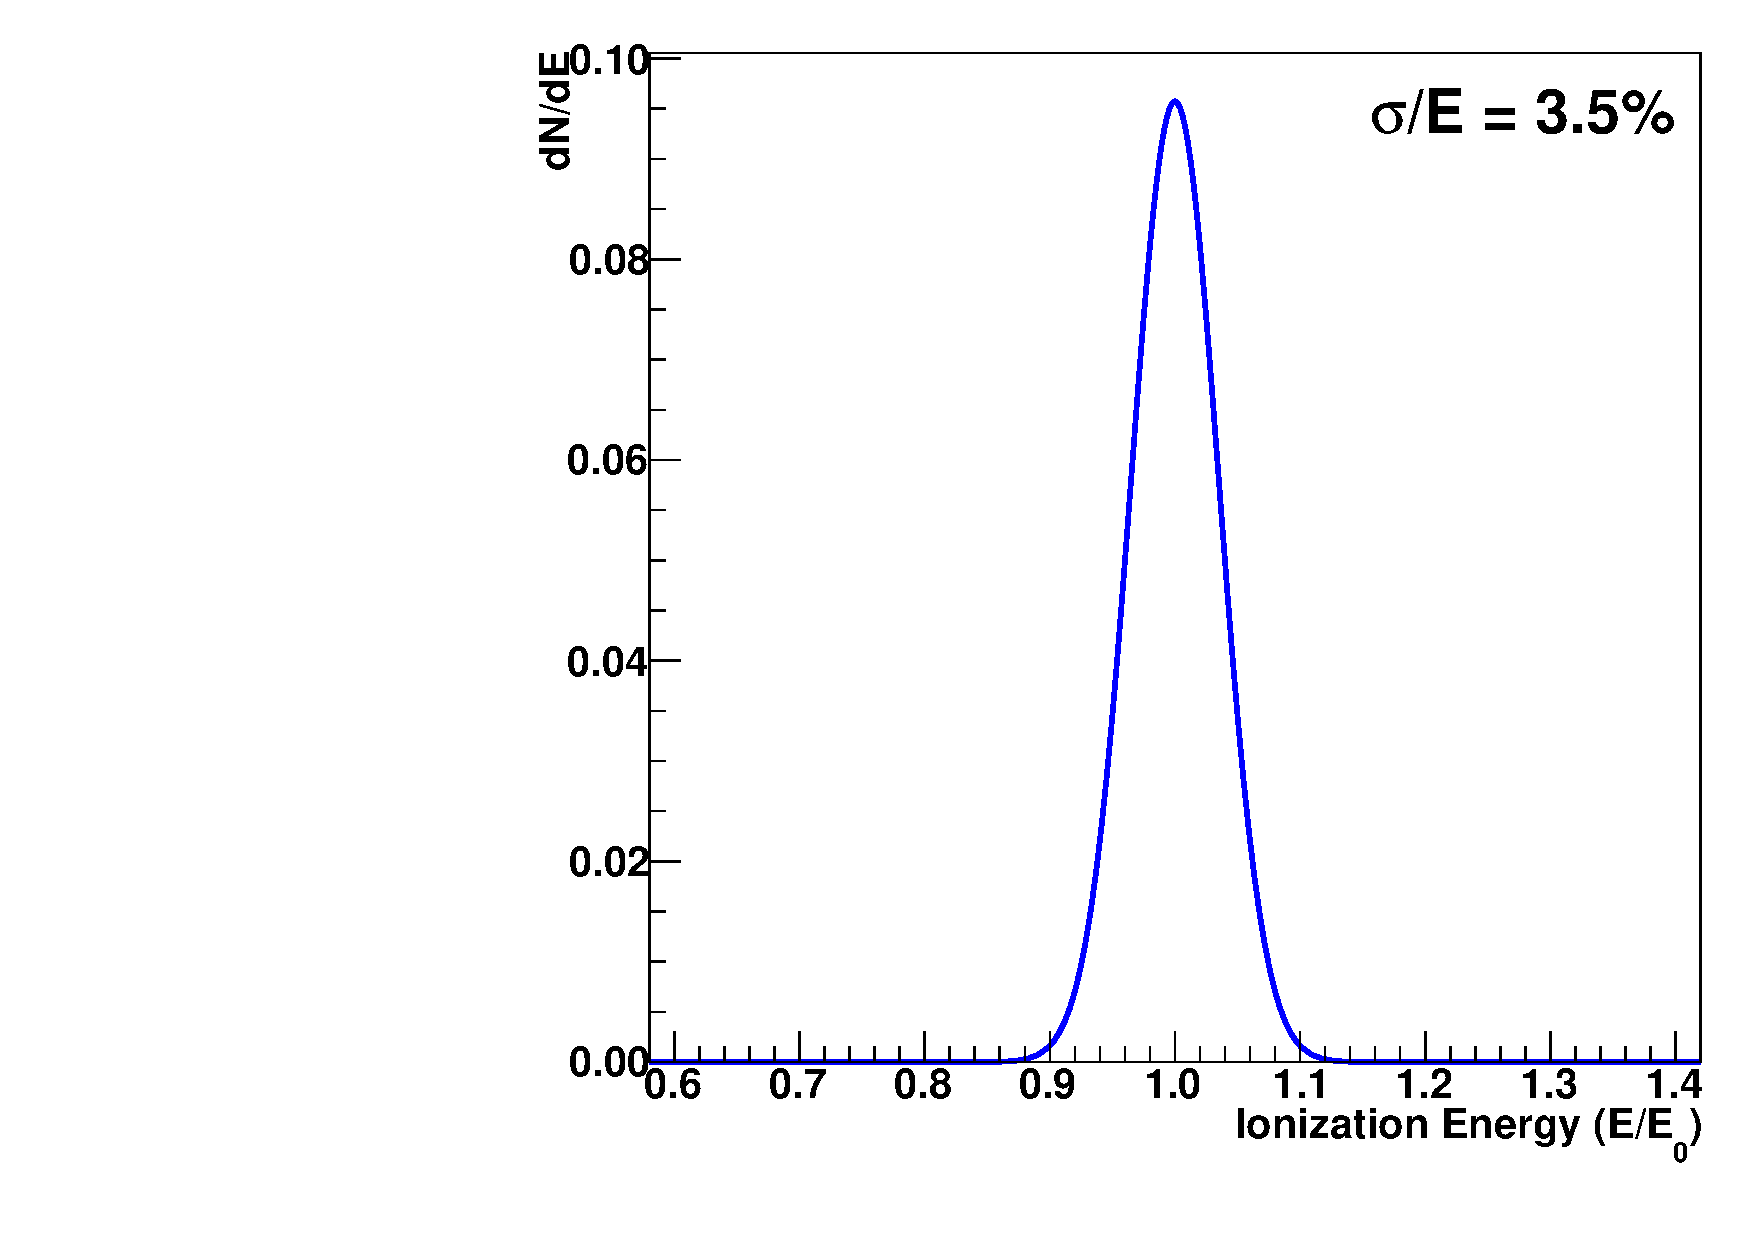
\includegraphics[width=\textwidth]{./plots/lxe_anticorrelation_ioniz.pdf}
\end{subfigure}\hspace{0.05\linewidth}\hfill%
\begin{subfigure}[c]{0.45\linewidth}
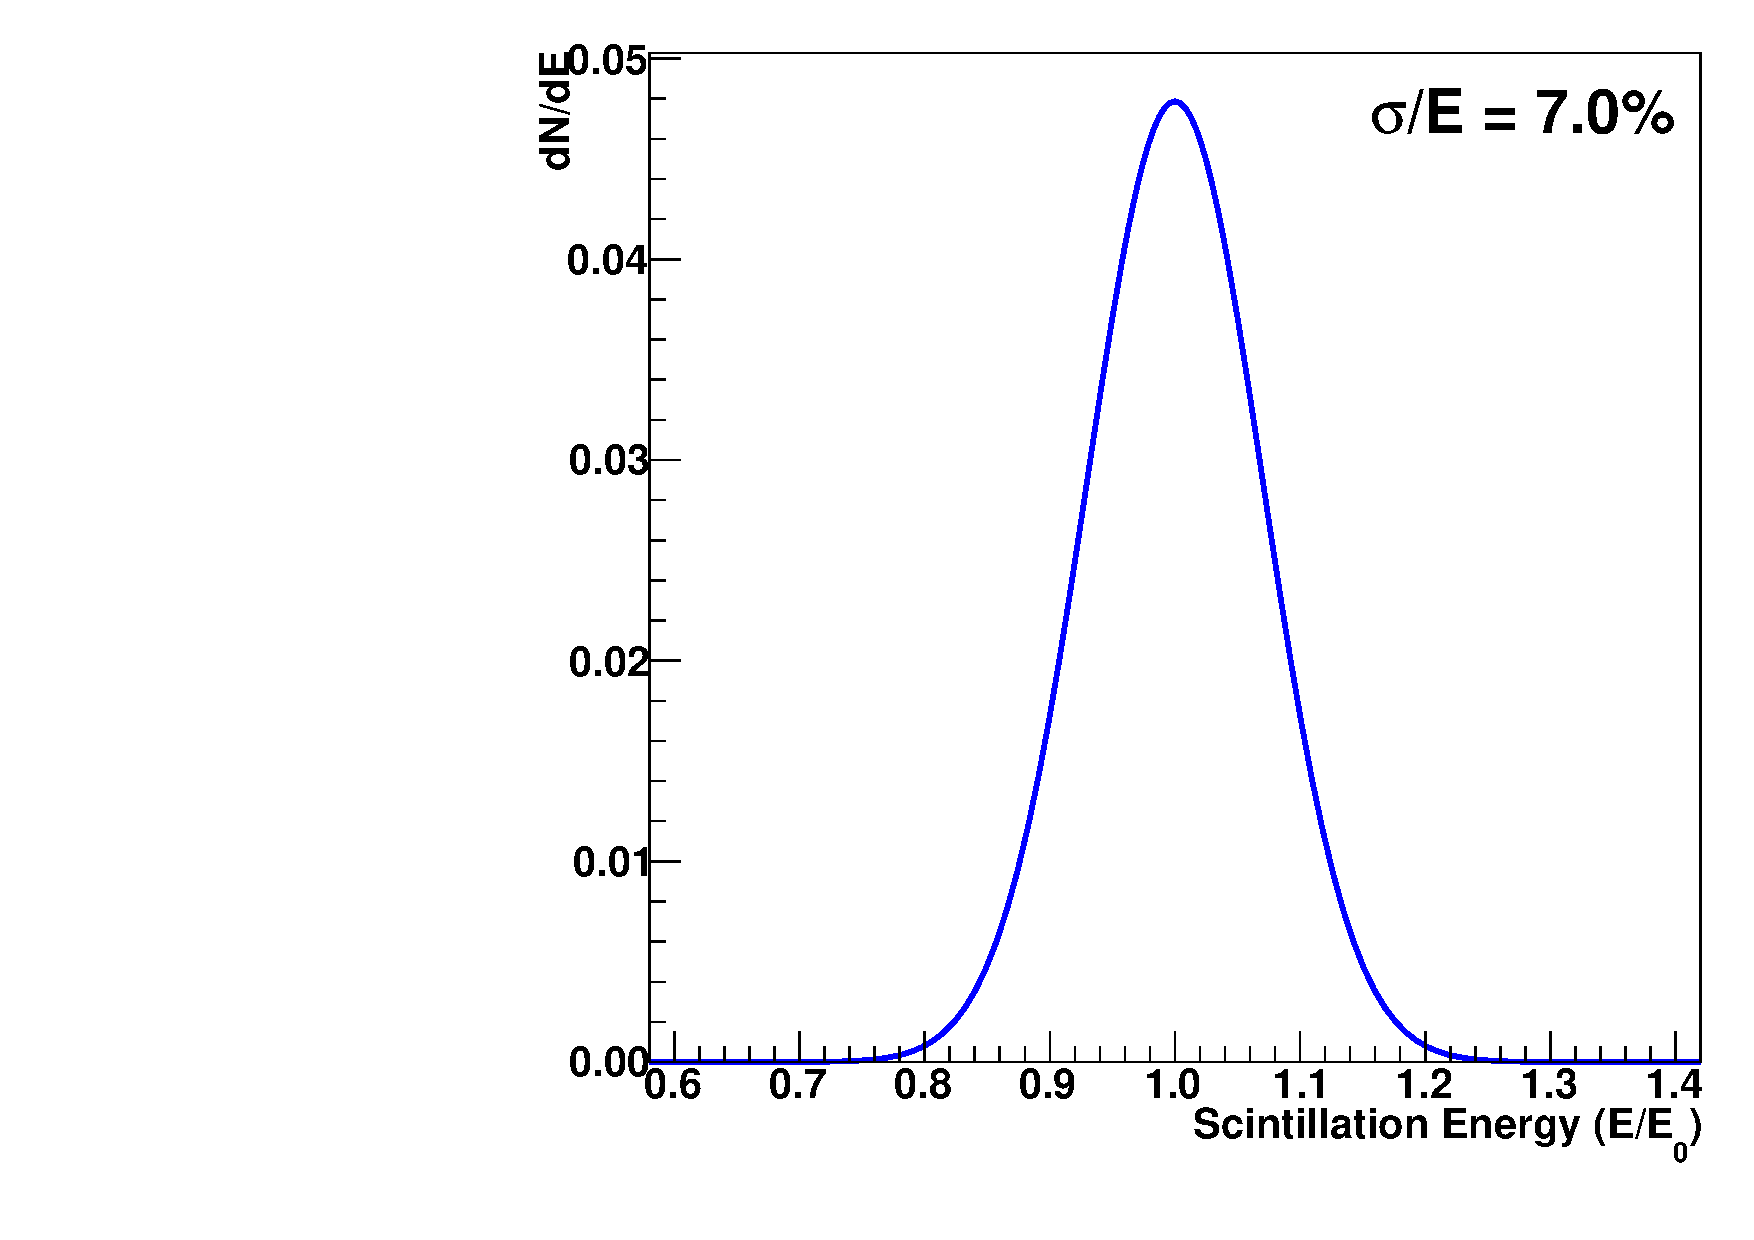
\includegraphics[width=\textwidth]{./plots/lxe_anticorrelation_scint.pdf}
\end{subfigure}
\begin{subfigure}[c]{0.45\linewidth}
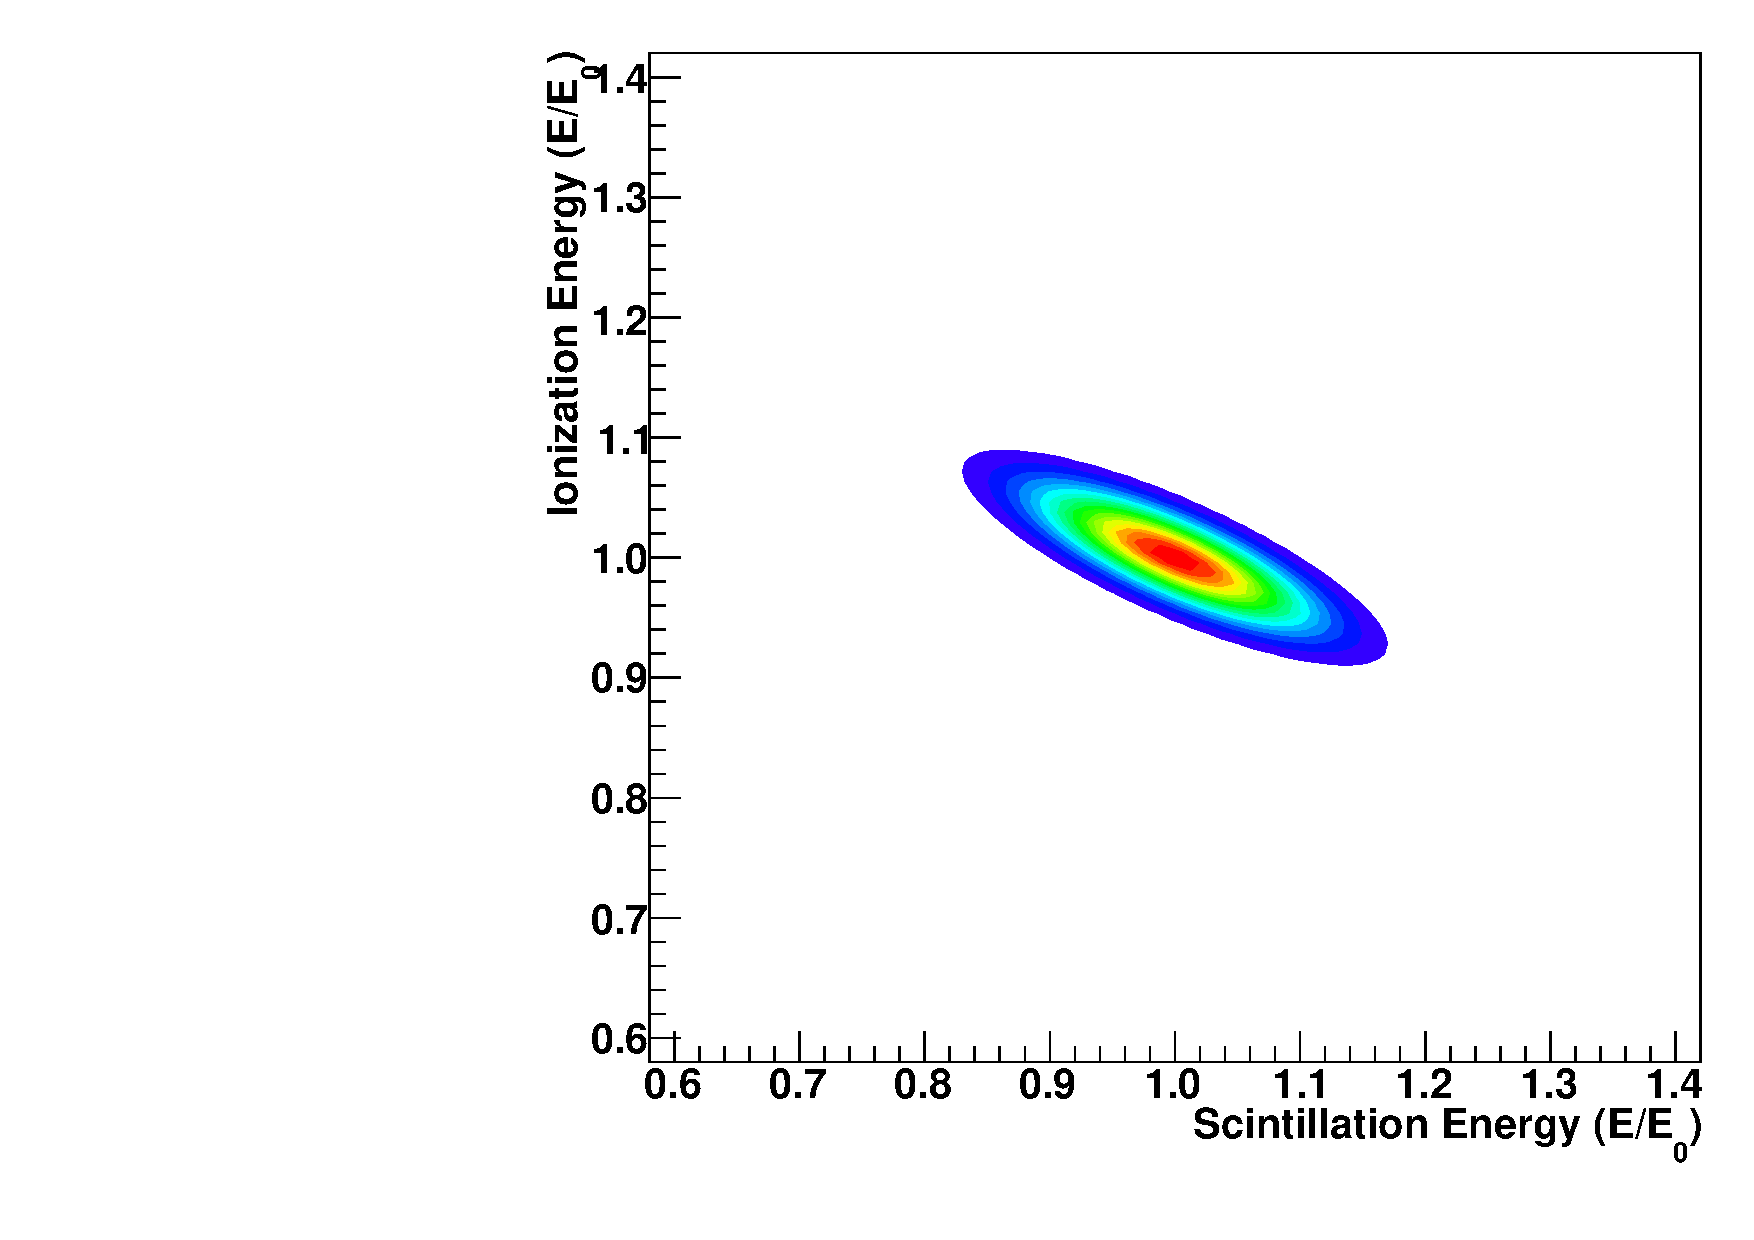
\includegraphics[width=\textwidth]{./plots/lxe_anticorrelation_2d.pdf}
\end{subfigure}\hspace{0.05\linewidth}\hfill%
\begin{subfigure}[c]{0.45\linewidth}
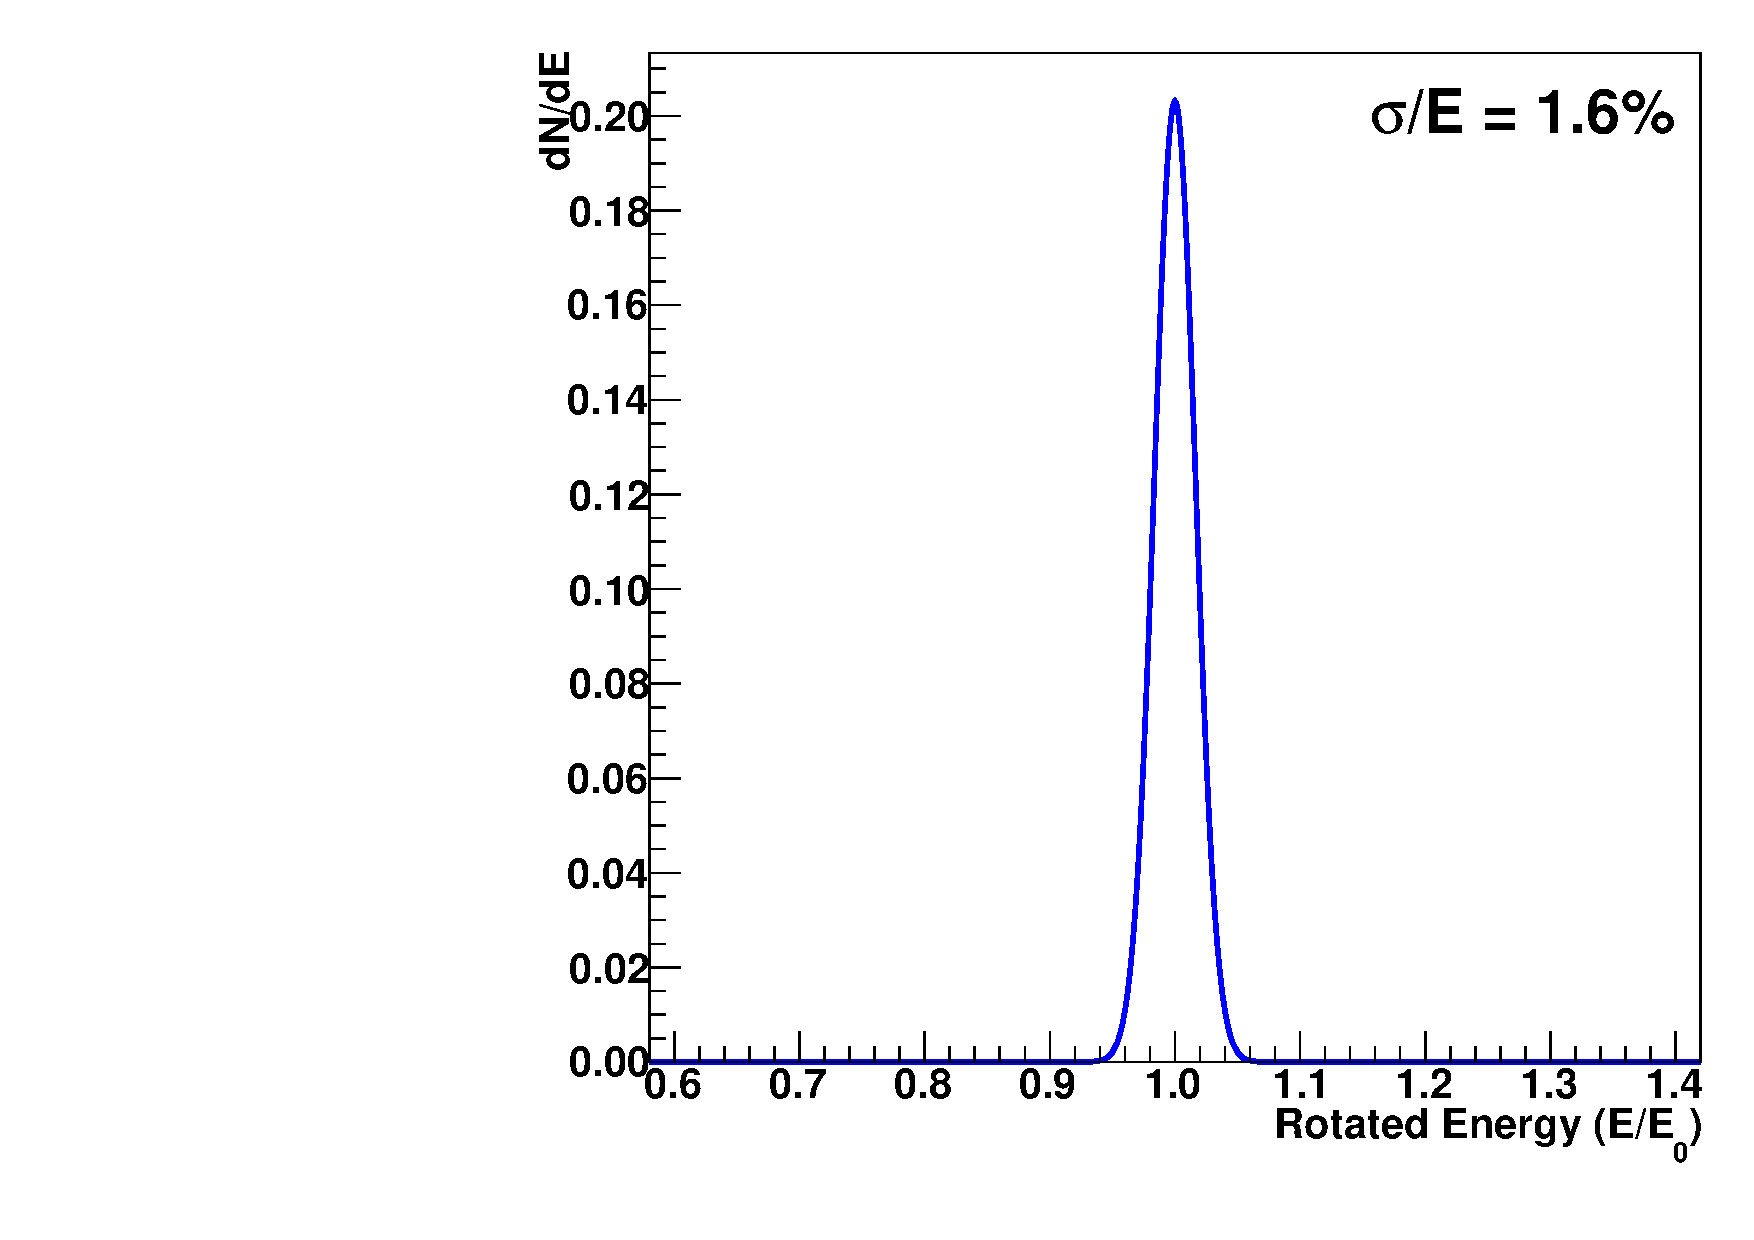
\includegraphics[width=\textwidth]{./plots/lxe_anticorrelation_rot.pdf}
\end{subfigure}
\caption[Anticorrelated Energy Resolution in Liquid Xenon]{A toy example of how the energy resolution of a monoenergetic line can be improved by combining signals in liquid xenon. The ionization signal (top left) and the scintillation signal (top right) show poor energy resolution individually. When the signals are anticorrelated (shown bottom left, with coefficient -0.8), they can be protected onto a rotated axis to yield an improved energy resolution (bottom right).}
\label{fig:toy_anticorrelation}
\end{figure}

\end{document}